\documentclass[tikz,border=2pt]{standalone}
\usepackage{tikz,pgfplots,pgf}
\usetikzlibrary{decorations.pathmorphing,decorations.text,calc}
\newcommand{\MYPI}{3.14159}
\newcommand{\MYTHETA}{25}
\newcommand{\MYSCALE}{4}
\newcommand{\XSHIFT}{0}
\newcommand{\OPRIME}{0}
\newcommand{\LINEPT}{2pt}
\definecolor{myblue}{rgb}{0.0,0.447,0.741}
\definecolor{myblue2}{rgb}{0.301,0.745,0.933}
\definecolor{myorange}{rgb}{0.85,0.325,0.098}
\definecolor{mygreen}{rgb}{0.466,0.674,0.188}
\definecolor{mypurple}{rgb}{0.494,0.184,0.556}
\definecolor{myred}{rgb}{0.635,0.078,0.184}
\definecolor{myyellow}{rgb}{0.929,0.694,0.125}
\begin{document}
	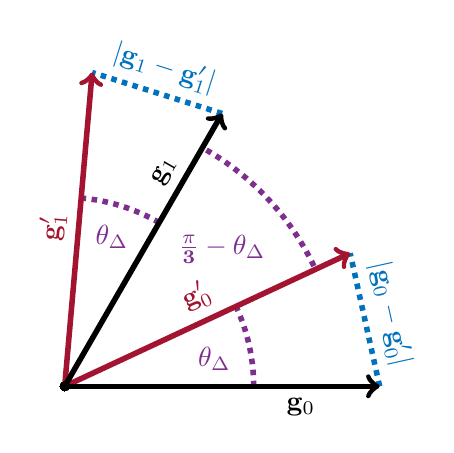
\begin{tikzpicture}\label{fig:k_vec}
	
		%%
			
		\coordinate (o1) at (0,0) ;
		\coordinate (g1) at ({1*\MYSCALE},0); 
		\coordinate (g2) at ({0.5*\MYSCALE},{0.866*\MYSCALE}); 
		
		\coordinate (h1) at ({\XSHIFT + (\OPRIME+cos(\MYTHETA))*\MYSCALE},{\MYSCALE*sin(\MYTHETA)}); 
		\coordinate (h2) at ({\XSHIFT + (\OPRIME+cos(\MYTHETA+60))*\MYSCALE},{\MYSCALE*sin(\MYTHETA+60)});  
		
		%%
		\draw[-,color=mypurple,dotted,line width=\LINEPT] ({0.6*\MYSCALE},0)  arc(0:\MYTHETA:0.6*\MYSCALE);
		\draw[-,color=mypurple,dotted,line width=\LINEPT] ({0.6*\MYSCALE*cos(60)},{0.6*\MYSCALE*sin(60)})  arc(60:85:0.6*\MYSCALE);

		\draw[-,color=mypurple,dotted,line width=\LINEPT] ({1.8},{3.0})  arc(60:\MYTHETA:0.85*\MYSCALE);
		
		\node (name) at ({0.475*\MYSCALE},{0.4*\MYSCALE*sin(0.5*\MYTHETA)}) {\color{mypurple} $\mathbf{\theta}_\Delta$};
		\node (name2) at ({0.3*\MYSCALE*cos(60)},{0.475*\MYSCALE*sin(\MYTHETA + 60)}) {\color{mypurple} $\mathbf{\theta}_\Delta$};
		\node (name1) at ({0.5*\MYSCALE},{0.8*\MYSCALE*(sin(0.5*(\MYTHETA))) + \MYPI/3}) {\color{mypurple} $\mathbf{\frac{\pi}{3}}-\theta_\Delta$};
		
		
		

		


		\draw[-,color=myblue,dotted,line width=\LINEPT] (g1) -- (h1) node  [midway, sloped, above] (TextNode) {\color{myblue}$|\mathbf{g}_{0} - \mathbf{g}^\prime_{0}|$};
		\draw[-,color=myblue,dotted,line width=\LINEPT] (g2) -- (h2) node  [midway, sloped, above] (TextNode) {\color{myblue}$|\mathbf{g}_{1} - \mathbf{g}^\prime_{1}|$};
		
	
		
				\draw[->,color=myred,solid,line width=\LINEPT] (o1) -- (h1) node  [midway,above, sloped] (TextNode) {\color{myred}$\mathbf{g}^\prime_{0}$};
		\draw[->,color=myred,solid,line width=\LINEPT] (o1) -- (h2) node  [midway,above, sloped] (TextNode) {\color{myred}$\mathbf{g}^\prime_{1}$};
	\draw[->,color=black,solid,line width=\LINEPT] (o1) -- (g1) node  [near end, below, sloped] (TextNode) {\color{black}$\mathbf{g}_{0}$};
		\draw[->,color=black,solid,line width=\LINEPT] (o1) -- (g2) node  [near end, above, sloped] (TextNode) {\color{black}$\mathbf{g}_{1}$};
		\draw[mark options={color=black},mark size=1.5\LINEPT] plot[mark=*] (o1);

		%%
		
%		\draw[dashed,->,color=myred,thick] (o2) -- (l1) node [midway, above, sloped] (TextNode) {$\mathbf{k_{22}}$};
%		\draw[dashed,->,color=myred,thick] (o2) -- (l2) node [midway, above, sloped] (TextNode)  {$\mathbf{k_{21}}$};
%		\draw[dashed,->,color=myred,thick] (o2) -- (l3) node [midway, above, sloped] (TextNode)  {$\mathbf{k_{23}}$};
%		\draw[mark options={color=myred},mark size=1pt] plot[mark=*] (o2);

	\end{tikzpicture}
\end{document}
